% =============================================================================
% sections/design/rover/hardware_overview.tex  -  Hardware Overview
% Teams: electronics (best guess - unconfirmed) / Status: EXAMPLE (scope approximation)
%
% EXAMPLE CONTENT for scope/layout approximation - not final report text.
% Adapted from the Preliminary Report's "System Architecture Wiring
% Diagram" subsection, trimmed to minimal prose. Marked with \exampleflag
% on its heading in the assembler.
%
% Image is a placeholder (figures/hardware_architecture.png) - swap it for
% the real wiring diagram by overwriting the same file. Shared figures/
% (not a team folder) since this is a whole-rover, system-level diagram.
% =============================================================================

The rover's onboard hardware is organized around a main computer that
performs high-level processing and sensor collection, primarily over USB,
coordinating with subsystem controllers over CAN and Ethernet: a chassis
controller drives the wheels, an arm controller manages actuators, sensors,
and the arm context camera, and dedicated science and operation subsystems
handle sampling instruments and external communication. The resulting
wiring architecture is shown in \autoref{fig:hardware_architecture}.

\begin{figure}[!htbp]
    \centering
    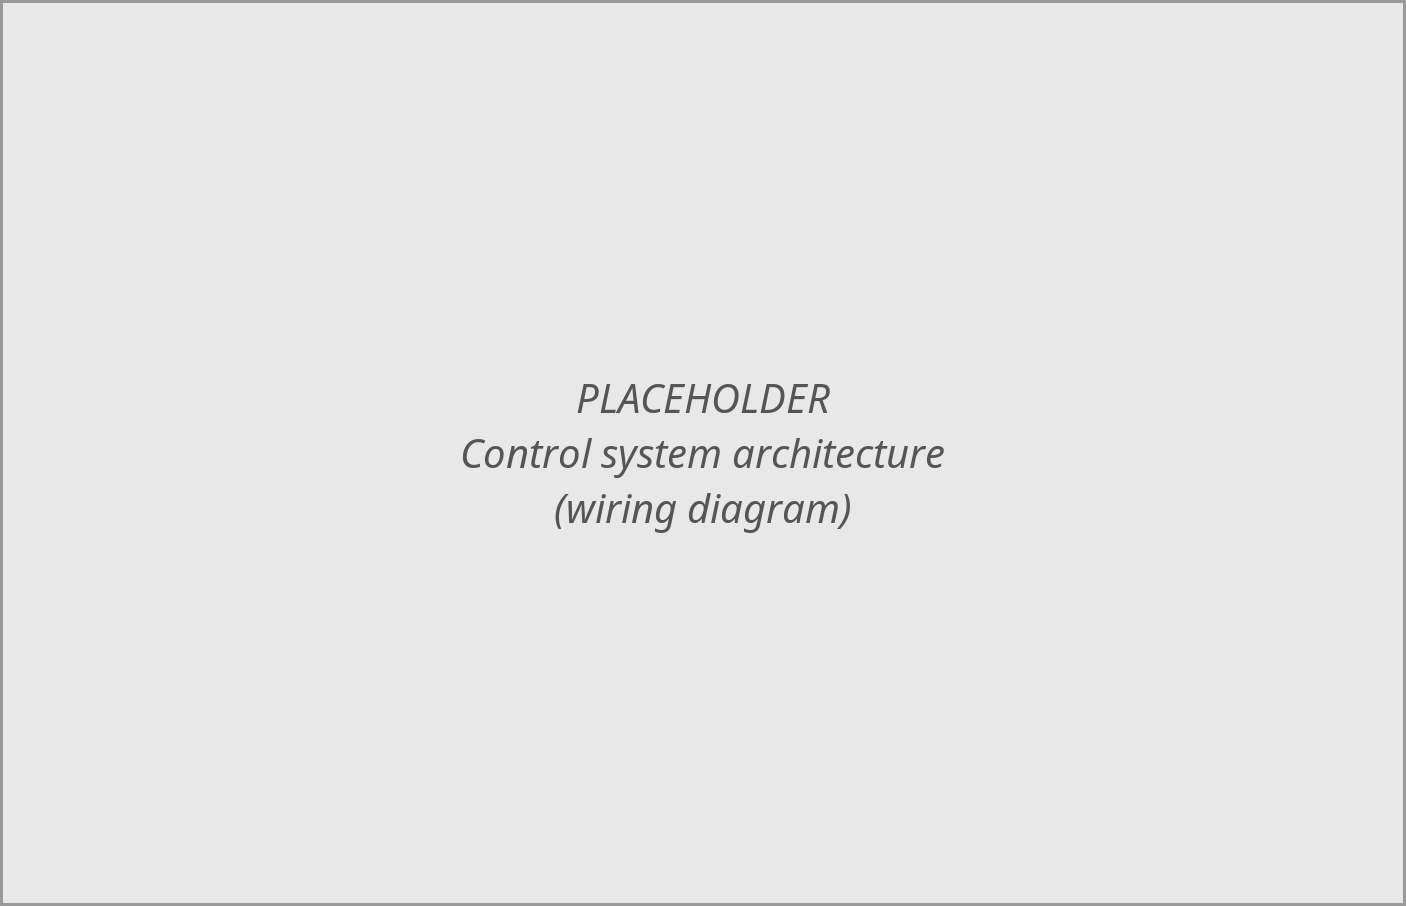
\includegraphics[width=0.85\linewidth]{figures/hardware_architecture}
    \caption{Control system architecture}
    \label{fig:hardware_architecture}
\end{figure}
